\chapter{Motivation}
\label{ch:motivation}

\section{Introduction}

\newthought{Increasingly frequent reports of antimicrobial resistance and immune escape} have lead to worries about a "post-antibiotic era": a time when common pathogens no longer respond to drugs and for which no effective vaccines exist\cite{WorldHealthOrganization:2014ug}.  For influenza A, a single serine to asparagine amino acid substitution (S31N) alters the properties of the $M_2$ ion channel\cite{Wang:1993uc}, interferes with the action of the adamantane class of antiviral drugs, and has reached fixation in the population\cite{Nelson:2009en}.  In \textit{Mycobacterium tuberculosis}, a four-year \textit{in vitro} drug challenge experiment on nine drug-susceptible isolates from a single patient demonstrated the strain could acquire resistance to nearly all first-line and most second-line drugs through just $12$ single nucleotide polymorphisms (SNPs)\cite{Eldholm:2014ei}.  \textit{Staphylococcus aureus} is the most common cause of post-operative infection worldwide and is increasingly unresponsive to $\beta$-lactam treatment and drugs in the penicillin group (methicillin, dicloxacillin, nafcillin, oxacillin, etc.).  Sequencing of methicillin-susceptible (MSSA) in the penicillin group and resistant (MRSA)\footnote{The term "methicillin resistant" is used in the literature, though it is taken to mean all drugs - including more stable variants of methicillin used in modern clinical practice} strains reveals the acquisition of resistance genes via mobile genetic elements and horizontally transferred genomic islands (e.g. the SCC\textit{mec} cassette chromosome upon which the methicillin and other $\beta$-lactam antibiotic resistance gene, \textit{mecA}, resides)\cite{Holden:2004kd}.

\textit{De novo} mutations (DNM), genomic variants arising anew in a sample and absent from progenitors, underlie many medically relevant pathogenic phenotypes.  The examples above all involve virulence phenotypes arising from spontaneous point mutations, structural variants, or horizontal gene transfer - all mutational methods that occur outside methods of traditional reproduction.  They are critical tools for pathogenic evolution and come in myriad forms.

\section{\textit{De novo} mutations (DNMs) in \textit{Plasmodium falciparum}}

\begin{table}[]
\centering
\caption{Phenotypes of \textit{P. falciparum} isolates used for genetic crosses.}
\label{tb:pf_phenotypes}
\begin{tabular}{@{}rcccccc@{}}
\toprule
                                 & 3D7 & HB3 & DD2 & 7G8 & GB4 & 803 \\
\midrule
pyrimethamine sensitivity        & -   & +   &     &     &     &     \\
chloroquine sensitivity          &     & +   & -   &     &     &     \\
infects mosquitoes easily        &     & +   & -   &     &     &     \\
infects \textit{Aotus nancymaae} &     &     &     & -   & +   & -   \\
artemisinin sensitivity          &     &     &     &     & +   & -   \\
\bottomrule
\end{tabular}
\end{table}

Experimental crosses of \textit{Plasmodium falciparum} parasites, the causative agent for the most deadly form of malaria, have enabled the discovery of a number of inherited and \textit{de novo} virulence factors.  The contrasting phenotypes for various strains of \textit{P. falciparum} are listed in Table \ref{tb:pf_phenotypes}.  For inherited factors, crossing of the pyrimethamine-resistant 3D7 and sensitive HB3 strains~\cite{Walliker:1987cv} revealed a nonsynoymous point mutation in the \textit{dhfr-ts}\footnote{dihydrofolate reductase-thymidylate synthase} gene, inhibiting binding of (and thus conferring resistance to) the drug~\cite{Peterson:1988wt}.  Analysis of the HB3 x DD2 cross\cite{Wellems:1990eg}, the latter of which is resistant to chloroquine, localized the determinant to a previously undetected gene on chromosome $7$, labelled \textit{pfcrt}\footnote{\textit{P. falciparum} chloroquine resistance transporter}, a member of a new family of transporters.  Additional investigation into differences in mosquito infection efficacy revealed down-regulation of the \textit{pfmdv-1}\footnote{\textit{P. falciparum} male gametocyte development gene 1} gene~\cite{Vaidya:1995up,Furuya:2005jn}, disruption of which results in marked reduction of mature and functional male gametocytes.

For uninherited factors, cytoadherence and antigenic properties of parasites facilitate evasion from host immune attack, and can differ substantially from the properties of their progenitors.  In 2000, Freitas-Junior \textit{et al.} showed that some 3D7 x HB3, HB3 x DD2, and HB3 x HB3 progeny harbored non-parental forms of subtelomeric \textit{var} genes, key members of an antigenic gene family\cite{FreitasJunior:2000cp}.  These altered forms were likely generated during mitosis by non-allelic homologous recombination\footnote{sometimes referred to as "ectopic" (aberrant) recombination in the literature} (NAHR) of telomeres from two different chromosomes\cite{Duffy:2009cc}.  The resulting genes are novel, functional, and never before observed by the host immune system.

These DNMs are critical tools for malaria to evade drug and immune pressure.  NAHR can further diversify a pathogen's antigenic repertoire, enabling continued evasion of immunological actors.  Duplications of a transporter gene may enable faster drug clearance in a parasite, thus conferring resistance.  Spontaneous point mutations may alter the binding site of a drug to a receptor, thus conferring immunity. 

\subsection{A reference-based approach for DNM discovery and genotyping}

With the advent of sequencing technologies, it is now straightforward to discover many DNMs.  Long reads (\textasciitilde $500$ bp) from the first-generation sequencing technology, Sanger sequencing, can be stitched together \textit{in silico} by considering the overlaps of sequences generated from many copies of the genome\cite{Myers:1995vma}.  This has enabled the reconstructions of full-length genomes and subsequent gene annotations for a single representative (or "reference") individual in a population.  Second-generation sequencing is leveraging economies of scale to reduce sequencing costs by several orders of magnitude\cite{Mardis:2011cr}.  The reads it produces are shorter (\textasciitilde $100$ bp) and more error-prone, but billions of them can be produced quickly.  Like the long reads, the short read data can also be assembled into a new genome, albeit with more errors and gaps, owing to the difficulty of overcoming large repetitive regions with short genomic fragments\cite{Schatz:2010if}.  Alternatively, assuming the sequence for the reference genome and a new individual are highly similar, it is far more common (and computationally more efficient) to align the reads to the reference\cite{Flicek:2009dl}.  String matching algorithms that allow mismatches, insertion, and deletions to appear in the alignments allow millions of sequnced reads to be placed on the reference genome quickly.  Separate tools can then examine the alignments, looking for the presence of non-reference alleles, and using statistical approaches to call and genotype variants with high accuracy\cite{Nielsen:2011kz}.

Variant calling software has been successfully applied to many sequencing datasets for the discovery of DNMs.  These variant callsets have provided insight into the development of drug resistance\cite{Woodford:2007it}, the genetic architecture of some common diseases\cite{Neale:2012ki}, and mutational rates in humans and chimpanzees with a strong paternal age effect\cite{Conrad:2011eh,Venn:2014ep,Kloosterman:2015cn,Francioli:2015kj}.  Many groups have released sophisticated software packages to facilitate these analyses and detailed instructions on their use\cite{DePristo:2011fo,Rimmer:2014ho}.

\subsection{A reference-free approach for assessing DNM sensitivity}

Specificity and sensitivity are crucial metrics to consider for any variant callset.  There are many approaches to establishing the specificity of a DNM callset.  For select variants (typically on the order of \textasciitilde $100$ variants from a callset), Sanger sequencing, Sequenom assays, and even targeted third-generation sequencing (i.e. PacBio sequencing, which can generate reads up to \textasciitilde $50,000$ bp as of this writing) have been used successfully to validate mutations.  Establishing sensitivity is much more difficult.  In theory, one would need complete and error-free reference genomes for both parents and each child in which the mutation calls are made.  Except for the smallest genomes, such an approach is prohibitively expensive.

Instead, it may be possible to establish the sensitivity of the reference-based protocol by considering how DNMs alter the genome of a sample with respect to its progenitors.  Consider a site where a DNM - say, a single SNP - has occurred, as depicted in Figure \ref{fig:kmer_venn}.  Although a single base of the genome has been altered, when the genome is divided into fixed-length words of length $k$, or "kmers", we find $k$ kmers that are present in the child but absent in the parents.  In this manner, DNMs can be considered generators of "novel" kmers - kmers present in the child but absent in the parents.  These kmers can be used as a signal to indicate the presence of a \textit{de novo} variant.  By choosing $k$ to be reasonably large so as to avoid analyzing short sequences that pervade the genome (half to two-thirds the length of a read will suffice), we can simply count continuous stretches of novel kmers as a proxy for the number of DNMs.

\begin{figure}[h!]
  \centering
    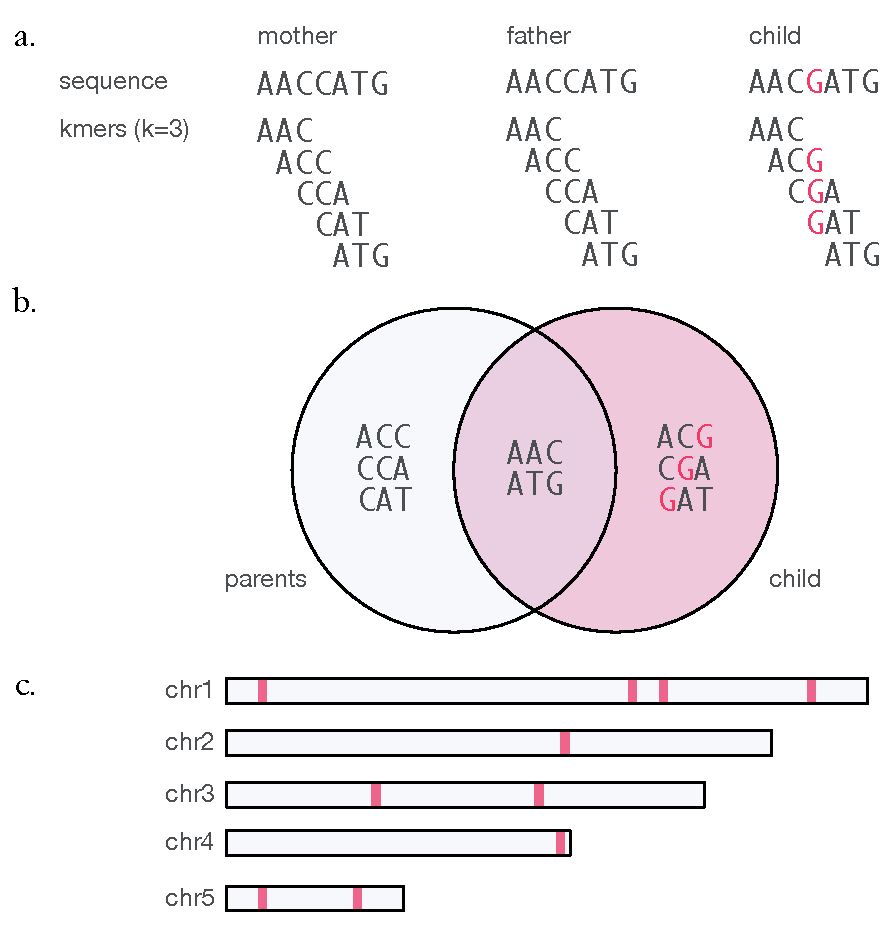
\includegraphics[width=\textwidth]{kmer_venn}
  \caption{a. Parental and child sequences at the site of a \textit{de novo} mutation, and the kmers generated at $k=3$.  b. The resulting Venn diagram of kmers found exclusively in the parents, the child, or common to both.  c. Novel kmers found around the genome indicate the presence of a \textit{de novo} mutation.}
  \label{fig:kmer_venn}
\end{figure}

This approach gives us a powerful, reference-free mechanism to verify the results of the reference-based analysis.  Sequencing of the whole genome is independent of any reference sequence that may already exist for the sample, and given sufficient coverage (Table \ref{tb:lw_cov} shows the requirements, assuming $76$ bp reads and a $23$ megabase genome), the raw data from a sequencing experiment should contain the full set of DNM-generated novel kmers, regardless of any mapping issues\cite{Lander:1988bp}.  Taking the reads that map, calling \textit{de novo} variants, and extracting the novel kmers from the immediate vicinity should theoretically reproduce that set.  Comparing the expected (reference-free) set to the observed (reference-based) kmer set should thus provide the sought sensitivity measure.

\begin{table}[]
\centering
\caption{Theoretical percentage of the genome recovered at a target depth of coverage.}
\label{tb:lw_cov}

\begin{tabular}{llll}
\toprule
coverage & numReads & numNucleotides & pctGenome\\
\midrule
1 & 302631 & 2.3e+07 & 63.21\\
2 & 605263 & 4.6e+07 & 86.47\\
3 & 907894 & 6.9e+07 & 95.02\\
4 & 1210526 & 9.2e+07 & 98.17\\
5 & 1513157 & 1.15e+08 & 99.33\\
6 & 1815789 & 1.38e+08 & 99.75\\
7 & 2118421 & 1.61e+08 & 99.91\\
8 & 2421052 & 1.84e+08 & 99.97\\
9 & 2723684 & 2.07e+08 & 99.99\\
10 & 3026315 & 2.3e+08 & 100.00\\
11 & 3328947 & 2.53e+08 & 100.00\\
12 & 3631578 & 2.76e+08 & 100.00\\
13 & 3934210 & 2.99e+08 & 100.00\\
14 & 4236842 & 3.22e+08 & 100.00\\
15 & 4539473 & 3.45e+08 & 100.00\\
16 & 4842105 & 3.68e+08 & 100.00\\
17 & 5144736 & 3.91e+08 & 100.00\\
18 & 5447368 & 4.14e+08 & 100.00\\
19 & 5750000 & 4.37e+08 & 100.00\\
20 & 6052631 & 4.6e+08 & 100.00\\
\bottomrule
\end{tabular}


\end{table}

\section{DNM sensitivity of the reference-based approach}

We now demonstrate these ideas on real data sets that will be used throughout this dissertation: experimental crosses between malaria parasites (\textit{Plasmodium falciparum}). %, and a two-generation pedigree of human's closest extant ancestor (and susceptible to \textit{falciparum} malaria), chimpanzees (\textit{Pan troglodytes})\footnote{Note that, while chimpanzees are used as an \textit{in vivo} model for the malaria parasite's liver stage in the production of the crosses, these two datasets are not related to one another.}.

The datasets that we'll be referring to in this work are summarized in Table \ref{tb:cross_info}.  For simplicity, we shall focus on the samples from the 3D7xHB3 cross.

\begin{table}[]
\centering
\caption{The \textit{P. falciparum} datasets that will be referred to throughout this work.}
\label{tb:cross_info}
\begin{tabular}{@{}rcccc@{}}
\toprule
                  & 3D7xHB3      & HB3xDD2      & 7G8xGB4      & 803xGB4      \\
\midrule
progeny           & 16           & 39           & 41           & 34           \\
read length       & 76           & 76           & 76           & 100          \\
fragment size     & $304 \pm 32$ & $251 \pm 50$ & $295 \pm 23$ & $222 \pm 10$ \\
coverage          & $96 \pm 40$  &              &              &              \\
\bottomrule
\end{tabular}
\end{table}

\subsection{Data processing}
We first generated the list of expected novel kmers by processing the raw sequencing data for each sample with the \textit{de novo} assembly software, Cortex\cite{Iqbal:2012fx} at $k=47$, standard settings for other parameters, and no error cleaning.  We produced the initial list of putative novel kmers by selecting kmers present in a child but absent in both parents.  We further produced a "confident" list of novel kmers by imposing a kmer coverage threshold, automatically determined by a custom algorithm designed to find a local minimum on the LOESS regression of the coverage distribution, as shown in Figure \ref{fig:kmer_cov_dist}.  Finally, we produce a "trusted" list of novel kmers by removing kmers originating from possible contaminants, as determined by performing a BLAST search on the confident list and removing all non-\textit{Plasmodium} hits.  These steps ensure that the list of trusted novel kmers is very restrictive.

\begin{figure}[h!]
  \centering
    \includegraphics[width=\textwidth]{{{PG0063-C.ERR019060.kmerCovThreshold}}}
  \caption{Kmer coverage distribution for a single 3D7xHB3 progeny, PG0063-C.  Red line indicates non-parametric LOESS fit upon which the local minimum is detected.}
  \label{fig:kmer_cov_dist}
\end{figure}

We aligned each sample's reads to the PlasmoDB 9.0 release of the \textit{Plasmodium falciparum} genome\cite{Gardner:2002p1564,Aurrecoechea:2009hh} using BWA-MEM\cite{Li:2013wn}.  We followed data processing guidelines as specified in the Genome Analysis Toolkit (GATK) best-practices documentation\cite{DePristo:2011fo,McKenna:2010p535}, flagging duplicate reads so that they are ignored downstream, and recalibrating base quality scores using the MalariaGen data release on the crosses as a truth set\cite{huh}.  As recent guidance by the authors indicates the GATK's variant calling software has internalized the local indel realignment functionality, we opted to forego running this step separately.  We called variants across all $18$ samples (parents and progeny) simultaneously using the GATK's HaplotypeCaller with standard settings and a ploidy of $1$.

A complete and perfect variant callset details the alterations that must be performed on the reference sequence in order to generate the genome of the sequenced sample.  Unfortunately, it is typically not possible to obtain a perfectly sensitive and specific callset.  False positives and false negatives proximal to true positives may interfere with our ability to generate the true underlying haplotype sequence.  To bypass this problem, we did not filter the variant callset.  Instead, we combinatorically generate all possible subsets of variants found within $100$ bp of each other using a recursive strategy to leave single elements out of a given set of kmers, presented in Algorithm \ref{alg:all_subsets}.  This will certainly generate vastly more kmers than truly exist in the sample's genome.  However, as we are only interested in verifying that the variant-induced kmers are present in our trusted novel kmer set, this approach has the benefit of providing maximum sensitivity.

\begin{algorithm}
\caption{Given a set of variants, generate all possible subsets of variants}
\label{alg:all_subsets}
\begin{algorithmic}[1]
\Function{generateAllPossibleSubsets}{variants}
    \State $\textit{loos} \gets []$

    \For{$i \gets 0 \textrm{ to } length(variants)$}
        \State $\textit{loo} \gets []$

        \For{$j \gets 0 \textrm{ to } length(variants)$}
            \If{$i \neq j$}
                \State $\textit{loo.add(variants[j])}$
            \EndIf
        \EndFor

        \If{$\textit{loo.size()} \ge 0$}
            \State $\textit{loos.add(loo)}$
        \EndIf

        \If{$\textit{loo.size()} \ge 1$}
            \State $\textit{generateAllPossibleSubsets(loo)}$
        \EndIf
    \EndFor

    \State $\textit{return loos}$
\EndFunction
\end{algorithmic}
\end{algorithm}

\subsection{Results}

\begin{figure}[h!]
  \centering
    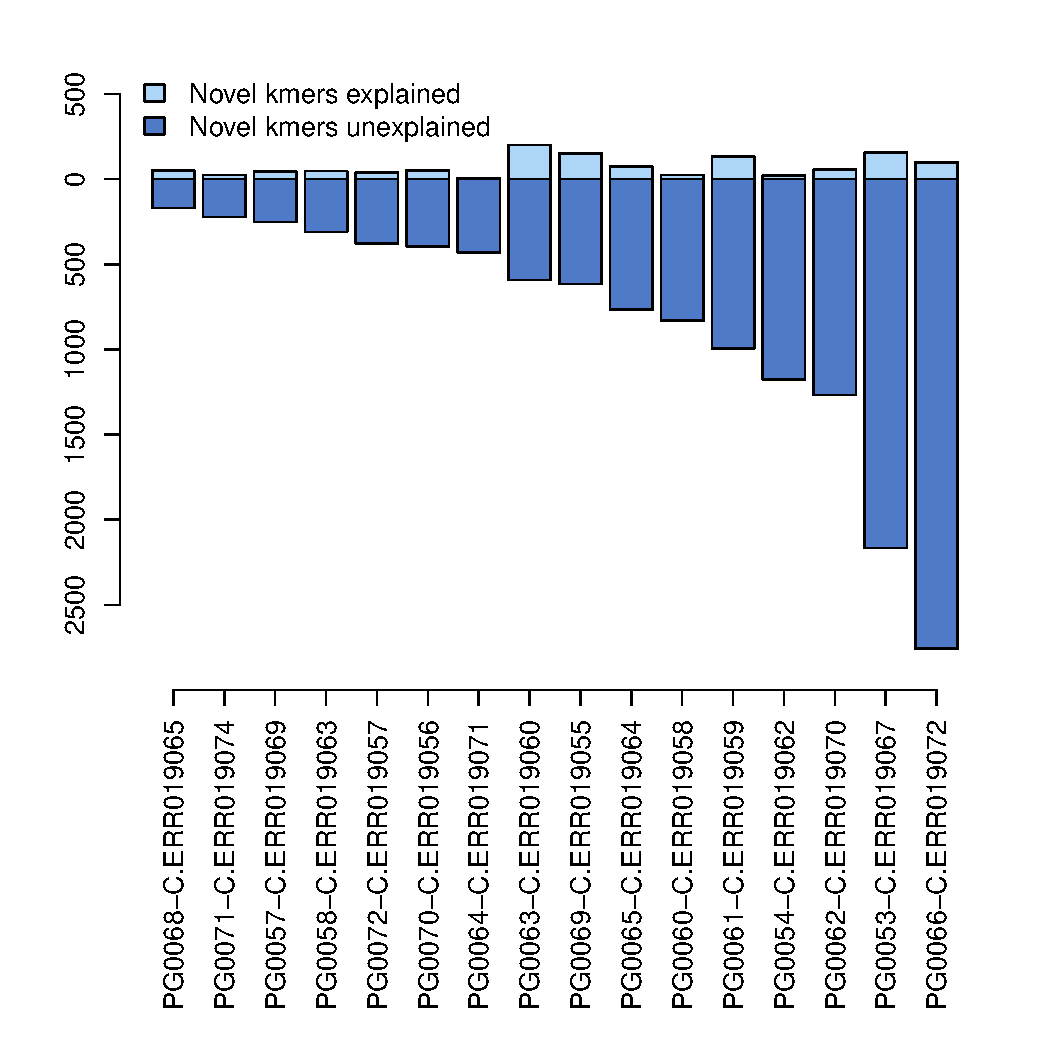
\includegraphics[width=\textwidth]{loadTables-1}
  \caption{Novel kmers observed in the reference-based analysis vs trusted novel kmers expected from the reference-free analysis.}
  \label{fig:obs_vs_exp_kmers}
\end{figure}

Figure \ref{fig:obs_vs_exp_kmers} shows the results of our reference-based vs reference-free analysis.  Per sample, our restrictive reference-free analysis has generated hundreds of trusted novel kmers to explain.  However, the reference-based analysis recapitulates only a fraction of these - only about $13\%$ on average.

Attempting to explain where these missing kmers have gone, we searched the reads for every trusted novel kmer.  More than $80\%$ of reads containing these kmers were found to map to multiple homes in the genome (summarized per sample in Figure \ref{fig:mapping}).

\begin{figure}[h!]
  \centering
    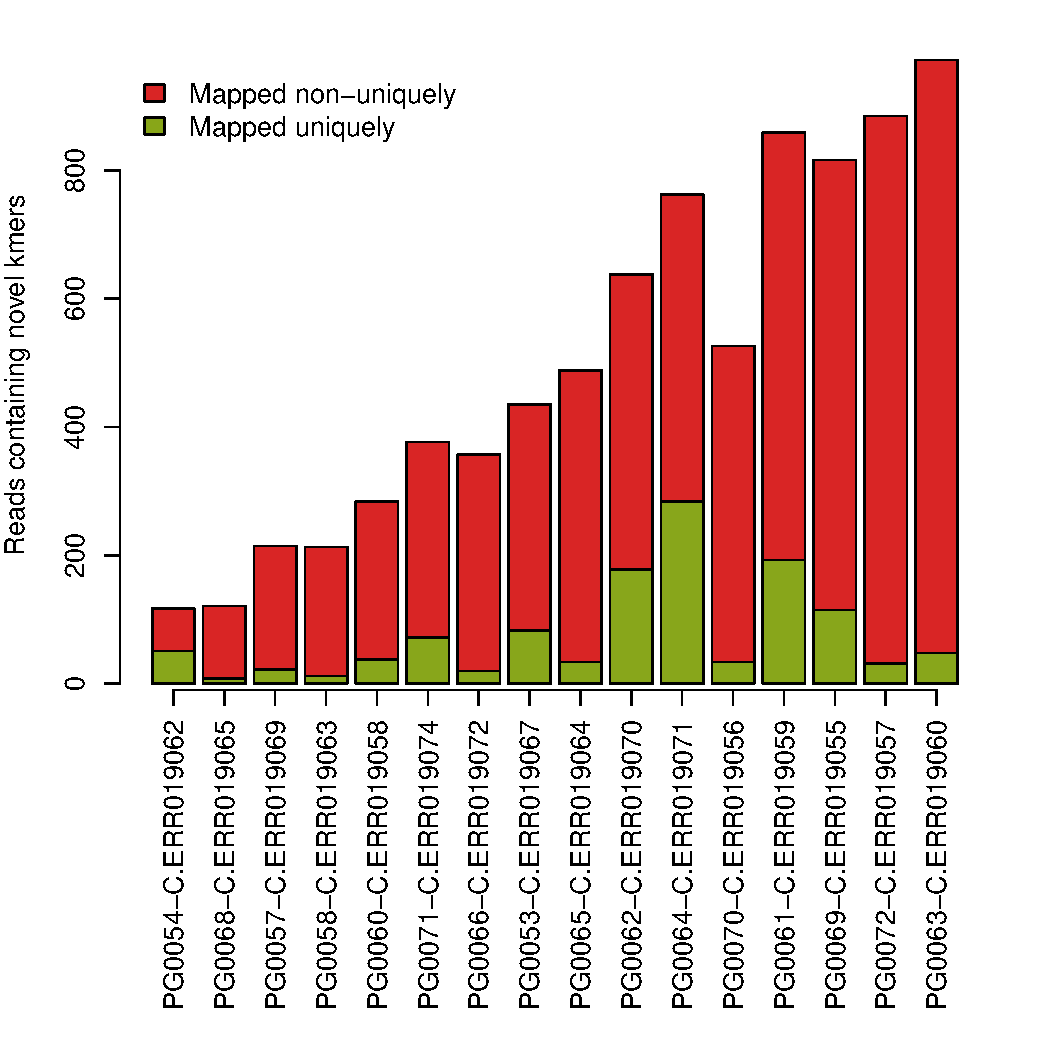
\includegraphics[width=\textwidth]{mapping-1}
  \caption{Reads that map once to the reference genome versus mapping multiple times, conditioned on the read containing a trusted novel kmer.}
  \label{fig:mapping}
\end{figure}

\section{Discussion}
\subsection{Failure of the mapping approach}

\begin{figure}[h!]
  \centering
    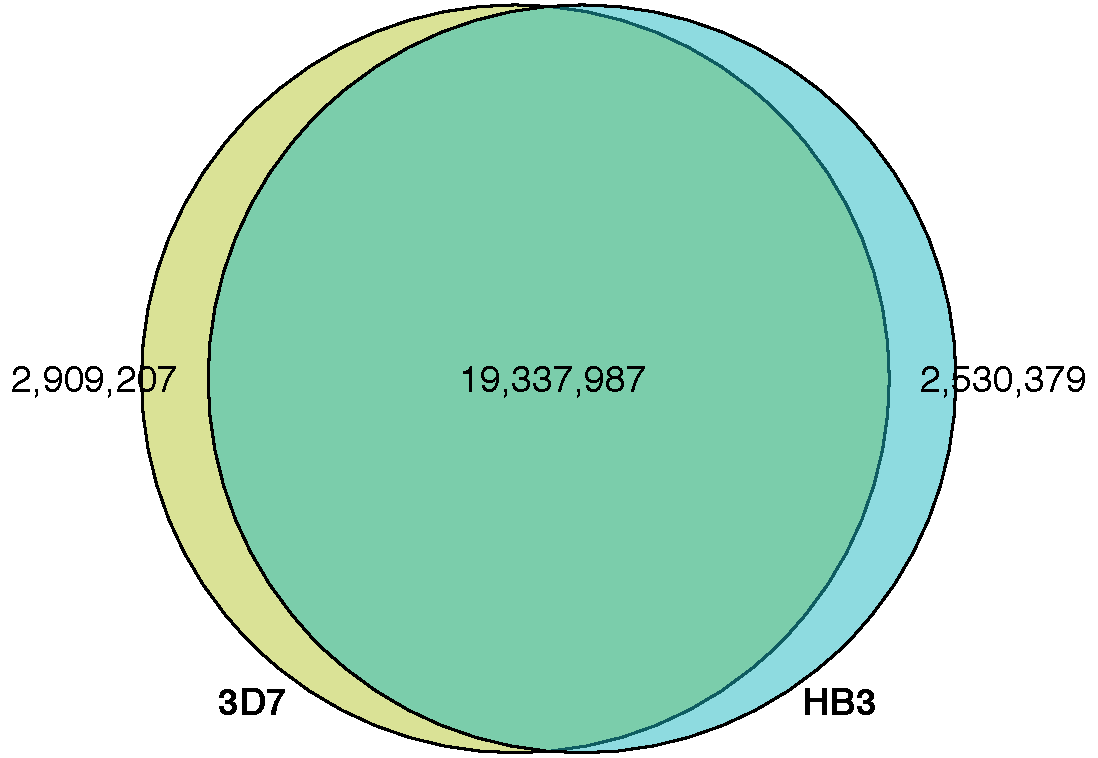
\includegraphics[width=\textwidth]{ref_venn_HB3}
  \caption{Venn diagram of kmers present in the 3D7 and HB3 genomes at $k=47$.  Both forward and reverse-compliment kmers are considered the same.}
  \label{fig:ref_venn_HB3}
\end{figure}

The preponderance of reads containing novel kmers fail to map uniquely to the reference genome, explaining why we should find such a massive discrepancy between the novel kmers we expect versus explain - reference-based calling approaches cannot call variants on unplaced reads.  That there should be so many reads that fail to map is perhaps not surprising, given the divergent nature of the reference genome to other samples.  Figure \ref{fig:ref_venn_HB3} shows the overlap between kmer sets between the 3D7 and HB3 genomes.  More than $20\%$ of the total set of kmers between these two samples is unique to each sample.

These unique kmers are not simply repetitive, intergenic, or otherwise uninteresting kmers.  They often reflect interesting biology.  Figure \ref{fig:kmer_recovery} shows one example: three \textit{var} genes from 3D7's $60$-member antigenic repertoire.  These genes do not overlap with the HB3 repertoire.  One of the 3D7xHB3 progeny, has inherited one of the 3D7 \textit{var} genes in full, but curiously exhibits mosaic recovery of two others.  This is known to be an NAHR event between the telomeres of chromosomes $1$ and $2$, likely to have occured during mitosis, preserving the domain architecture and yielding a functional product\cite{Claessens:2014fo}.

\begin{sidewaysfigure}[h!]
  \centering
    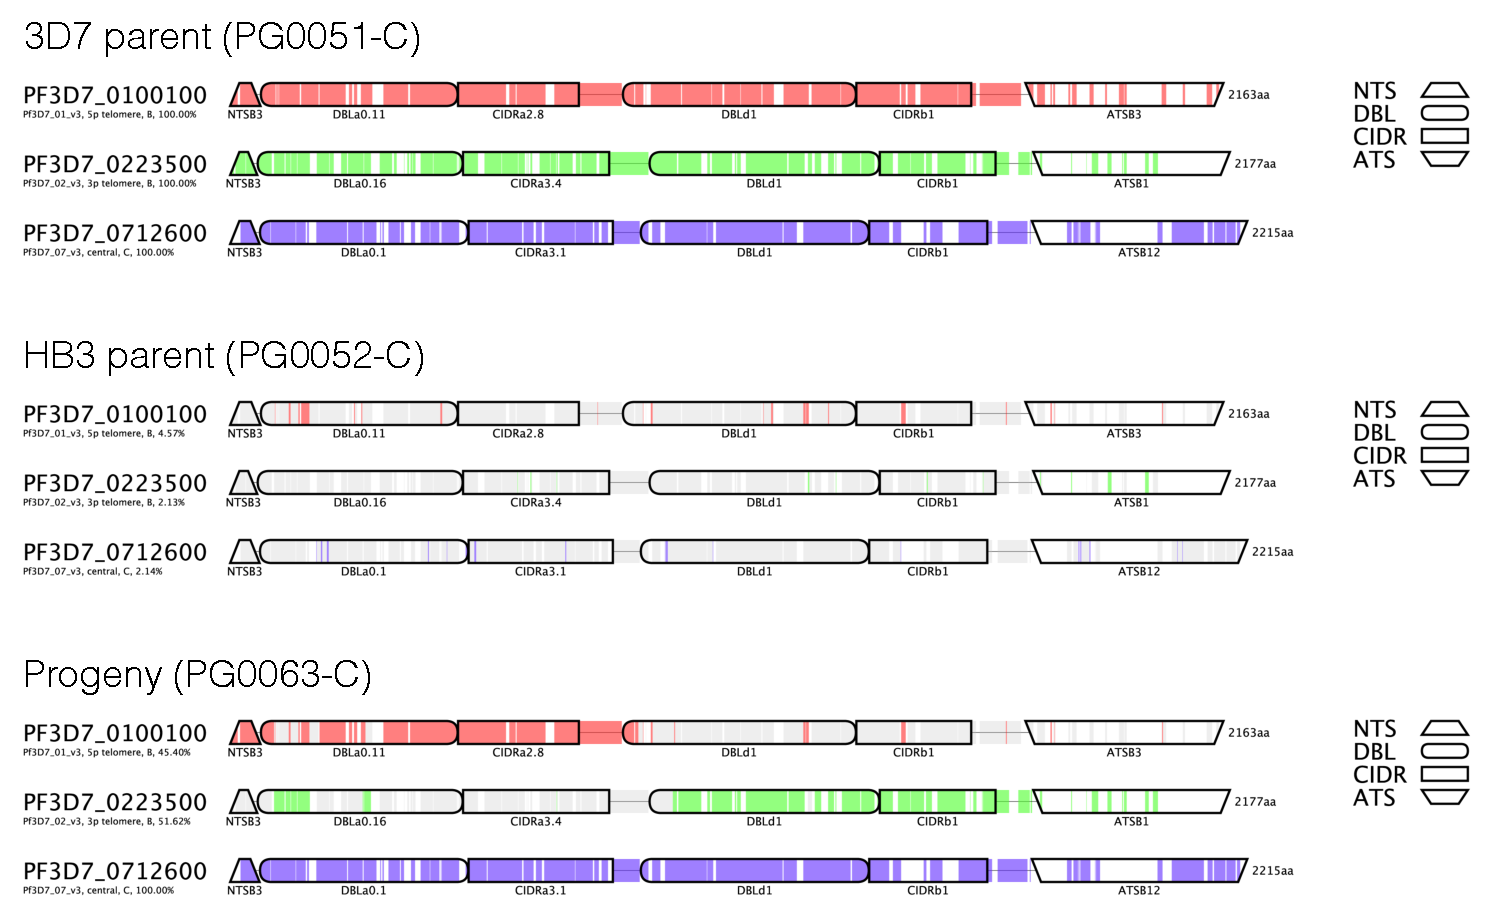
\includegraphics[width=\textwidth]{kmer_recovery}
  \caption{Presence and absence of unique kmers in three 3D7 \textit{var} genes.  Each vertical line represents a kmer.  Colored kmers represent those unique 3D7 kmers that are recovered in the sample.  Grey indicates no recovery.  White indicates the kmer at that position was not unique in the 3D7 genome.  Only the coding regions of the respective genes are shown, with domain annotations obtained from the VarDom server\cite{Rask:2010fia}.}
  \label{fig:kmer_recovery}
\end{sidewaysfigure}

Alignment of short reads to a single reference and subsequent application of variant callers is a poor strategy for \textit{de novo} variant discovery in \textit{P. falciparum} (and likely higher-order species as well) for a number of reasons:

\begin{enumerate}
\item \textbf{Absent or divergent loci in genome} \hfill \\ The underlying assumption that two genomes from the same species should be very similar is inappropriate for highly diverse populations (e.g. pathogens) or hypervariable regions (e.g. immune loci in mammals).  If a haplotype present in the sample is too dissimilar to the reference, or perhaps even completely absent, read aligners may return incorrect results.  Reads may align to the wrong location, the resultant mismatches mistaken for real mutations.  Alternatively, they may fail to align at all, thus obscuring evidence of real variation.

\item \textbf{Incomplete or errorful reference sequences} \hfill \\ Reference sequences are often incomplete and/or contain errors due to technical artifacts.  Chaisson \textit{et al.} provide an excellent review on the various errors that may arise\cite{Chaisson:2015dg}.  Regions of the genome may fail to amplify during library preparation, leading to coverage dropout and subsequent gaps in the assembly.  Insufficiently long reads used in the reference genome construction may lead to the misestimation of lengths of repetitive regions, causing repeats to have a collapsed representation relative to the true genome.  Segmental duplications, gene families, or other loci with high sequence identity may generate ambiguous read overlaps that cannot be resolved without very long reads.

\item \textbf{Difficult to include prior information about variation in a species} \hfill \\ Read aligners must make a decision as to how many apparent mismatches to permit with respect to the reference sequence.  However, these software packages typically operate per-read, without information on prior population variation throughout the genome.  

\item \textbf{Inability to include improved or project-specific data} \hfill \\ Improvements in sequencing technology, or new platforms altogether, can yield supplementary datasets that adds missing information to a genome or repairs a misrepresented locus.  There is no natural framework for incorporating these additional datasets to the alignment framework.
\end{enumerate}

\begin{figure}[b]
  \centering
    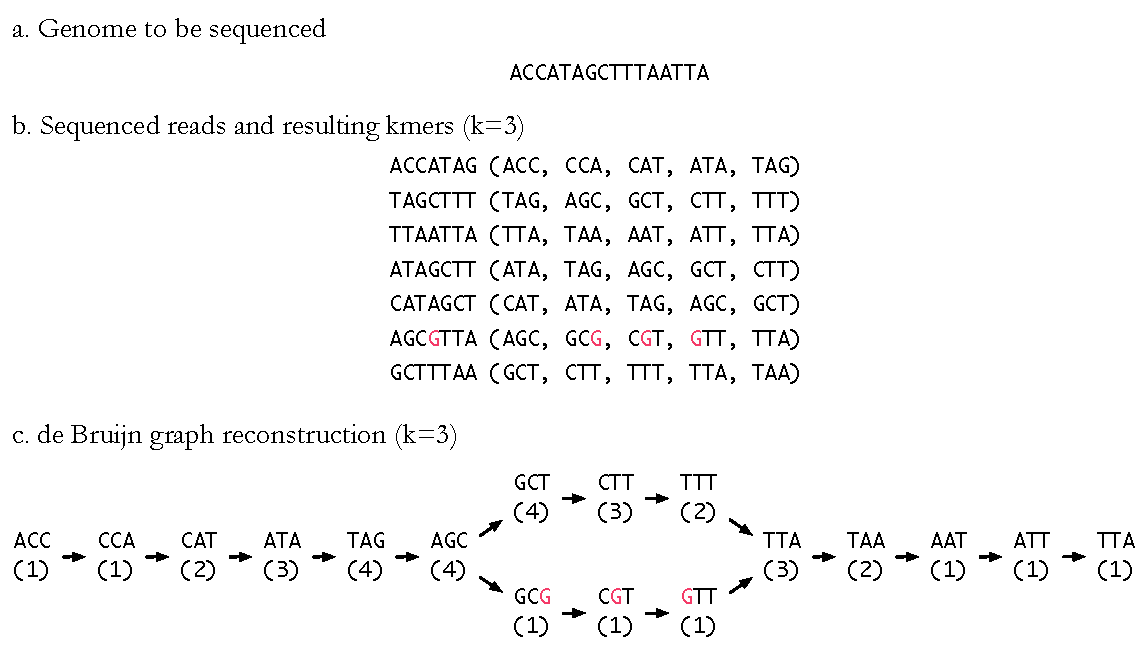
\includegraphics[width=0.7\textwidth]{debruijn}
  \caption{The process of generating a de Bruijn graph representation of sequence data.  a. The underlying genome. b. Reads sequenced from the genome (including one read with a sequencing error).  Reverse-complement reads are not shown for clarity.  c. The $k=3$ de Bruijn graph reconstruction, including kmer coverage annotations.}
  \label{fig:debruijn}
\end{figure}

\subsection{\textit{De novo} assembly as an alternative approach}

Consider Table \ref{tb:lw_cov} again, which demonstrates that we can expect to recover the full genome at as little as $10$-fold coverage.  For small genomes (\textit{P. falciparum} is approximately $23$ megabases in length), modern sequencing experiments can routinely return excess of $100$-fold coverage.  It is therefore clear that deeply-sequenced samples will have reads representing the entirety of the genome despite our inability to align all of them to the genome.  Rather than relying on mapping to an imperfect and incomplete reference, we can attempt to assemble the genome \textit{de novo} - from the sequenced data itself, ignoring the availability of a reference sequence.

The problem of performing \textit{de novo} assembly essentially reduces to computing read-to-read alignments, rather than read-to-reference alignments.  As each read represents recovery of some small region of the genome, the supersequence of overlapping reads (the aligned nucleotides flanked by the non-overlapping sequences from each read) represent some larger linear stretch of the genome.  Brute-force computation of all possible pairwise alignments is $\mathcal{O}(N^2)$ in the number of reads, which is impractical for second-generation sequencing datasets with tens or hundreds of millions of reads.  Fortunately, there are many ways to compute and represent these overlaps efficiently.  We shall focus on one $\mathcal{O}(N)$ method in this work: assembly via construction of a de Bruijn graph.

Formal definitions can be found below.  Informally, a graph is simply a data structure representing a collection of objects (termed "vertices" or "nodes") and connections ("edges" or "links").  In a de Bruijn graph, each vertex is a unique element.  Applied to sequencing, a de Bruijn graph encodes linear stretches of sequence, while each edge represents an overlap with the connected vertices.  Commonly, each read is decomposed into fixed-length words of an arbitrary length $k$, or "kmers".  As each kmer is sequentially extracted from a read and added to the graph as vertices, edges between adjacent kmers in the read are stored as well.  Overlapping reads will share kmers, and since each kmer can only appear once in the graph, adding kmers and edges from the overlapping read effectively records the alignment without needing to literally compute all possibilities.  Figure \ref{fig:debruijn} depicts a simple $16$ bp genome, sequenced with $7$ bp reads, and the resulting de Bruijn graph constructed at a kmer size of $3$.

Construction of this data structure is not without its challenges.  First, errors in second-generation sequencing data are very common, and therefore the graph produced from raw sequencing data will contain many branches that are not in the actual genome (examine Figure \ref{fig:debruijn} again, observing the highlighted base - a sequencing error - and the resultant perturbation to the otherwise linear graph).  These can be mitigated (but perhaps not completely solved) by error-cleaning algorithms that remove low coverage kmers, as presumably in high coverage data, random errors are rare and can be detected and discarded.  Second, long repetitive stretches of the genome that feature the same kmers multiple times will be collapsed into a single copy, as de Bruijn graphs only store each kmer once.  Finally, homology in the genome can cause two separate regions of the genome to appear proximal to one another in the graph.  This may result in a vertices with multiple outgoing edges, causing unresolvable ambiguity when traversing the graph.

Nevertheless, such an approach should resolve many of the deficiences of an alignment-based approach.  Absent or divergent loci should be recovered.  The uncleaned graph should be complete (barring any regions of the genome that suffer from an amplification bias that prevents them from being sequenced).  Prior information about variation in the species (or in this case, just the parents) are included by assembling the parents and comparing to them directly, rather than indirectly via the reference.  Finally, additional information can be added at graph construction time or by adding a separate color to the graph encoding the supplementary data.

\subsection{Formal definitions}

\begin{figure}[h!]
  \centering
    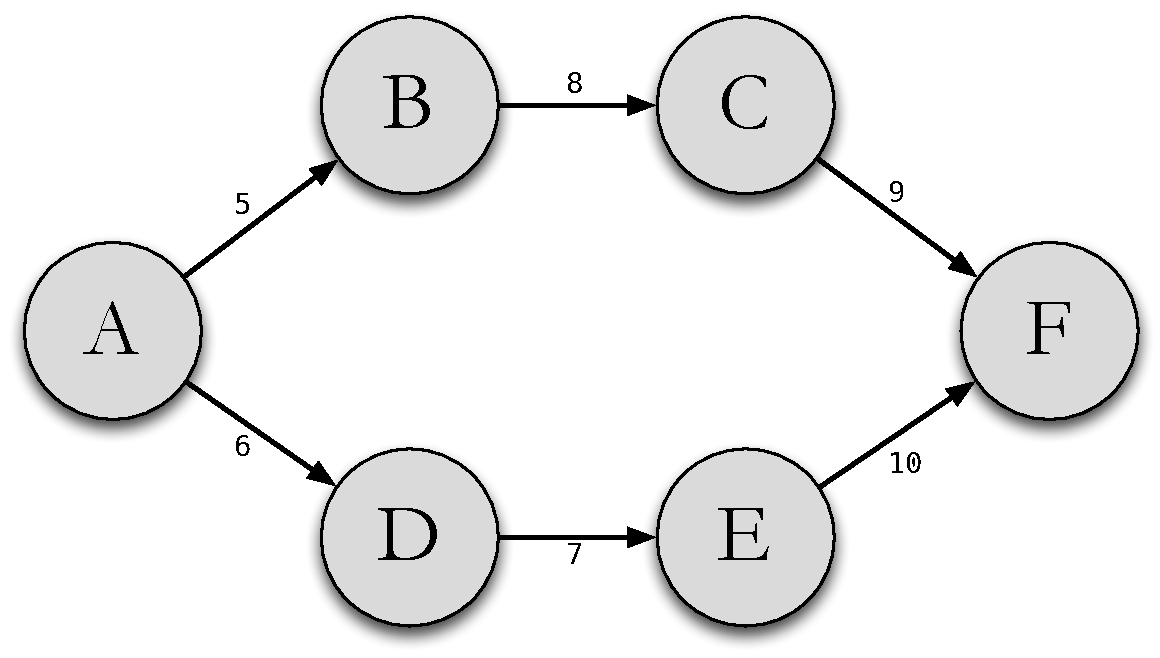
\includegraphics[width=\textwidth]{examplegraph}
  \caption{An example directed graph with six vertices.}
  \label{fig:examplegraph}
\end{figure}

We denote a \textbf{graph} as $G = \{\mathcal{V}, \mathcal{E}\}$ where $\mathcal{V}$ represents a unique set of \textbf{vertices}, and $\mathcal{E}$ a set of \textbf{edges}\cite{Koller:2009ty}.  We shall assume the set of vertices $\mathcal{V} = V_1, V_2, ..., V_n$.  A pair of vertices may be connected by an edge.  For the purposes of this dissertation, we shall require that all edges are \textbf{directed}, though generally, it is also possible for edges to be \textbf{undirected}.  Written as $V_i \rightarrow V_j$ or equivalently $V_j \rightarrow V_i$, directed edges restrict graph traversal in one direction (thus enforcing a traversal order when reconstructing a region of the genome).  A vertex may have a number of incoming (outgoing) edges, the precise count being referred to as a vertex's \textbf{in- (out-) degree}.

A \textbf{path} is a sequence of adjacent vertices that respects these edge relationships, i.e. $V_i, ..., V_k$ such that for every $j = i, ..., k$, we have $V_j \rightarrow V_{j+1}$.  In Figure \ref{fig:examplegraph}, the vertex sequence $A, B, C, F$ forms a path.  Similarly, a \textbf{trail} denotes a vertex sequence, but does not respect the directionality of the edges.  In Figure \ref{fig:examplegraph}, the sequence $F, E, D, A$ forms a trail.  Edges can carry weights, indicating an arbitrary cost for traversing from one vertex to another via particular edges.

A \textbf{multi-color graph} is a useful extension for multi-sample scenarios.  Each edge carries additional metadata used to denote sample identity (each sample is assigned a unique "color").  All kmers in all samples are added to the graph, and following the edges with the same color yields the genome of that sample.  Many kmers will not be accessible when traversing paths or trails in one color versus another.  These motifs are the hallmark of most variation in a graphical setting.

Often in this dissertation, we will perform operations on a limited graph region wherein we process only vertices of interest and all edges present between them in the original graph.  This is referred to as an \textbf{induced subgraph} (which is \textit{not} technically synonymous with a subgraph, but for simplicity in this work, we will often drop the "induced" qualifier).  Let $\mathbf{V} \subset \mathcal{V}$.  The \textbf{subgraph} $G[\mathbf{V}] = \{\mathbf{V}, \mathcal{E'}\}$ where $\mathcal{E'}$ are all the edges $V_i \rightleftharpoons V_j \in \mathcal{E}$ such that $V_i, V_j \in \mathbf{V}$.

\section{Overview of this work}

In this dissertation, we present a novel multi-color graph-based approach to \textit{de novo} mutation detection and allele identification.  We show how knowledge of the pedigree enables us to identify so-called \textbf{novel kmers} - kmers present in children and absent from parents - that serve as an exceedingly strong signal as to the presence of \textit{de novo} variation.  We use these kmers to analyze subgraphs in the genome likely to represent DNMs and navigate color-specific paths and trails to determine the precise allele.  We also demonstrate how the novel kmers act as "sign posts" during graph traversal, indicating that a traversal is following a fruitful path.  This simultaneously constrains th runtime of the algorithm and allows us to overcome sequencing error that could not otherwise be overcome.  We demonstrate that this approaches yields vastly superior sensitivity and specificity to DNMs than conventional methods, and can easily access events that occur on the haplotypic background of the non-reference parent.  

In Chapter 2, I present a review on mutational mechanisms that generate de novo mutations, their rates, factors that influence their generation, and known events in various species.

Chapters 3 and 4 detail the software packages I have written for this work, the former including descriptions of the realistic variant read simulations, the latter detailing the graph genotyping algorithm.

Chapters 5 and 6 present results from applying the algorithm to real data.  The former chapter focuses on the aforementioned \textit{P. falciparum} crosses.  The latter addresses a \textit{Pan troglodytes} pedigree.

Finally, Chapter 7 discusses the work in a larger context and details various improvements that can be made in future work.
